\documentclass[12pt, a4paper]{article}

% ── Packages ──────────────────────────────────────────────────────────────────
\usepackage[T1]{fontenc}
\usepackage[margin=2.5cm]{geometry}
\setlength{\headheight}{14pt}
\usepackage{lmodern}
\usepackage{microtype}
\usepackage{xcolor}
\usepackage{amssymb}
\usepackage{titlesec}
\usepackage{enumitem}
\usepackage{booktabs}
\usepackage{array}
\usepackage{tabularx}
\usepackage{listings}
\usepackage{tikz}
\usepackage{fancyhdr}
\usepackage{mdframed}
\usepackage{parskip}
\usepackage{setspace}
\usepackage[hypcap=false]{caption}
\usepackage{float}
\usepackage{hyperref}

\usetikzlibrary{shapes, shapes.geometric, arrows.meta, positioning, shadows.blur}

\setlength{\emergencystretch}{3em}

% ── Colours ───────────────────────────────────────────────────────────────────
\definecolor{darwinblue}{RGB}{52, 86, 150}
\definecolor{darwindark}{RGB}{25, 35, 65}
\definecolor{darwinlight}{RGB}{235, 241, 255}
\definecolor{darwinaccent}{RGB}{80, 120, 195}
\definecolor{okgreen}{RGB}{39, 174, 96}
\definecolor{termbg}{RGB}{15, 15, 20}
\definecolor{termtext}{RGB}{220, 220, 220}
\definecolor{termgreen}{RGB}{80, 200, 120}
\definecolor{termcyan}{RGB}{90, 190, 210}
\definecolor{termyellow}{RGB}{230, 195, 80}
\definecolor{codebg}{RGB}{246, 248, 252}
\definecolor{rulecol}{RGB}{52, 86, 150}
\definecolor{greytext}{RGB}{100, 100, 110}

% ── Hyperref ──────────────────────────────────────────────────────────────────
\hypersetup{
    colorlinks  = true,
    linkcolor   = darwinblue,
    urlcolor    = darwinblue,
    citecolor   = darwinblue,
    pdftitle    = {Darwin: A Privacy-Focused Research Agent},
    pdfauthor   = {Mohammad Ammar, Divya Vinaybhai Patel, Samantha Susan John},
    pdfborder   = {0 0 0}
}

% ── Section styling ───────────────────────────────────────────────────────────
\titleformat{\section}
  {\large\bfseries\color{darwindark}}
  {\thesection.}{0.6em}{}
  [\vspace{2pt}\color{rulecol}\rule{\linewidth}{1pt}]

\titleformat{\subsection}
  {\normalsize\bfseries\color{darwinblue}}
  {\thesubsection}{0.6em}{}

\titleformat{\subsubsection}
  {\normalsize\itshape\color{darwindark}}
  {}{0em}{}

\titlespacing{\section}{0pt}{20pt}{8pt}
\titlespacing{\subsection}{0pt}{14pt}{4pt}
\titlespacing{\subsubsection}{0pt}{10pt}{2pt}

% ── Header / Footer ───────────────────────────────────────────────────────────
\pagestyle{fancy}
\fancyhf{}
\fancyhead[L]{\small\color{greytext}Darwin --- Privacy-Focused Research Agent}
\fancyhead[R]{\small\color{greytext}Technical Report, 2026}
\fancyfoot[C]{\small\thepage}
\renewcommand{\headrulewidth}{0.4pt}

% ── Listings ──────────────────────────────────────────────────────────────────
\lstdefinestyle{terminal}{
    backgroundcolor  = \color{termbg},
    basicstyle       = \ttfamily\scriptsize\color{termtext},
    keywordstyle     = \color{termcyan}\bfseries,
    stringstyle      = \color{termgreen},
    commentstyle     = \color{greytext},
    breaklines       = true,
    breakatwhitespace= true,
    postbreak        = \mbox{\textcolor{greytext}{$\hookrightarrow$}\space},
    frame            = single,
    framerule        = 0pt,
    xleftmargin      = 8pt,
    xrightmargin     = 8pt,
    aboveskip        = 6pt,
    belowskip        = 6pt,
    showstringspaces = false,
    columns          = fullflexible,
    keepspaces       = true,
}

\lstdefinestyle{pycode}{
    backgroundcolor  = \color{codebg},
    basicstyle       = \ttfamily\scriptsize\color{darwindark},
    keywordstyle     = \color{darwinblue}\bfseries,
    stringstyle      = \color{okgreen!80!black},
    commentstyle     = \color{greytext}\itshape,
    breaklines       = true,
    frame            = leftline,
    framerule        = 2pt,
    rulecolor        = \color{darwinblue},
    xleftmargin      = 14pt,
    aboveskip        = 6pt,
    belowskip        = 6pt,
    showstringspaces = false,
    language         = Python,
}

% ── Helper commands ───────────────────────────────────────────────────────────
\newcommand{\code}[1]{\texttt{\small\color{darwinblue}#1}}
\newcommand{\done}{\textbf{\color{okgreen}$\checkmark$ Implemented}}

% ── Info / highlight box ──────────────────────────────────────────────────────
\newmdenv[
    backgroundcolor = darwinlight,
    linecolor       = darwinblue,
    linewidth       = 1.5pt,
    leftline        = true,
    rightline       = false,
    topline         = false,
    bottomline      = false,
    innerleftmargin = 12pt,
    innerrightmargin= 8pt,
    innertopmargin  = 7pt,
    innerbottommargin= 7pt,
    skipabove       = 8pt,
    skipbelow       = 8pt,
]{infobox}

% ══════════════════════════════════════════════════════════════════════════════
\begin{document}

% ── Title page ────────────────────────────────────────────────────────────────
\begin{titlepage}
\centering
\vspace*{2.5cm}

{\color{darwinblue}\rule{\linewidth}{2.5pt}}
\vspace{0.8cm}

{\Huge\bfseries\color{darwindark} Darwin}\\[0.4em]
{\LARGE\bfseries\color{darwinblue} A Privacy-Focused Research Agent}\\[0.3em]
{\large\color{greytext} Built on the Model Context Protocol}

\vspace{0.8cm}
{\color{darwinblue}\rule{\linewidth}{2.5pt}}
\vspace{1.8cm}

{\large\bfseries Mohammad Ammar \quad Divya Vinaybhai Patel \quad Samantha Susan John}

\vspace{0.6cm}
{\color{greytext} April 2026}

\vfill

\begin{mdframed}[
    backgroundcolor = darwinlight,
    linecolor       = darwinblue,
    linewidth       = 1pt,
    innerleftmargin = 18pt,
    innerrightmargin= 18pt,
    innertopmargin  = 12pt,
    innerbottommargin= 12pt,
]
\setlength{\parskip}{4pt}
\textbf{Abstract.}
Darwin is a fully local, privacy-preserving research assistant that connects a large language model running on Ollama to external academic tools through the Model Context Protocol (MCP). The system integrates an ArXiv MCP server for paper discovery and retrieval, a PDF parsing server for content extraction, and an Obsidian server for persistent knowledge management. A multi-turn agentic control loop drives autonomous literature review workflows, while a human-in-the-loop approval mechanism, local file caching, structured logging, and robust error handling make the pipeline production-ready. All computation and storage remain on the user's machine, with no data sent to external services beyond the arXiv API.
\end{mdframed}

\end{titlepage}

\tableofcontents
\newpage

% ══════════════════════════════════════════════════════════════════════════════
\section{Introduction}

Literature review is one of the most time-intensive steps in any research workflow. Researchers must search across databases, read and evaluate dozens of papers, extract relevant findings, and maintain structured notes --- all while ensuring that sensitive research topics and unpublished ideas are not unnecessarily exposed to cloud services.

Darwin addresses these challenges through a single, unified agent that runs entirely on the user's local machine. The system is built on three design principles:

\begin{enumerate}[leftmargin=2em, itemsep=4pt]
    \item \textbf{Privacy by default.} Papers are downloaded locally, PDFs are parsed locally, and the language model runs on local hardware via Ollama. No research queries or document contents are sent to external cloud inference endpoints.
    \item \textbf{Modularity through MCP.} The Model Context Protocol provides a standard interface between the language model and external tool servers. Each capability (arXiv search, PDF parsing, Obsidian notes) is an independent server that can be upgraded or replaced without modifying the orchestrator.
    \item \textbf{Agentic autonomy with human oversight.} The agent executes multi-step workflows autonomously but enforces a human-in-the-loop gate before downloading papers, ensuring the user retains control over what enters their local storage.
\end{enumerate}

The result is a system that can perform a full literature review --- search, filter, download, parse, summarise, and archive --- within a single conversational session, on a standard laptop, with no cloud dependencies beyond the public arXiv API.

% ══════════════════════════════════════════════════════════════════════════════
\section{System Architecture}

\subsection{Overview}

Darwin follows a layered, modular architecture. The three layers are kept strictly separate so that each can be tested and extended independently.

\begin{center}
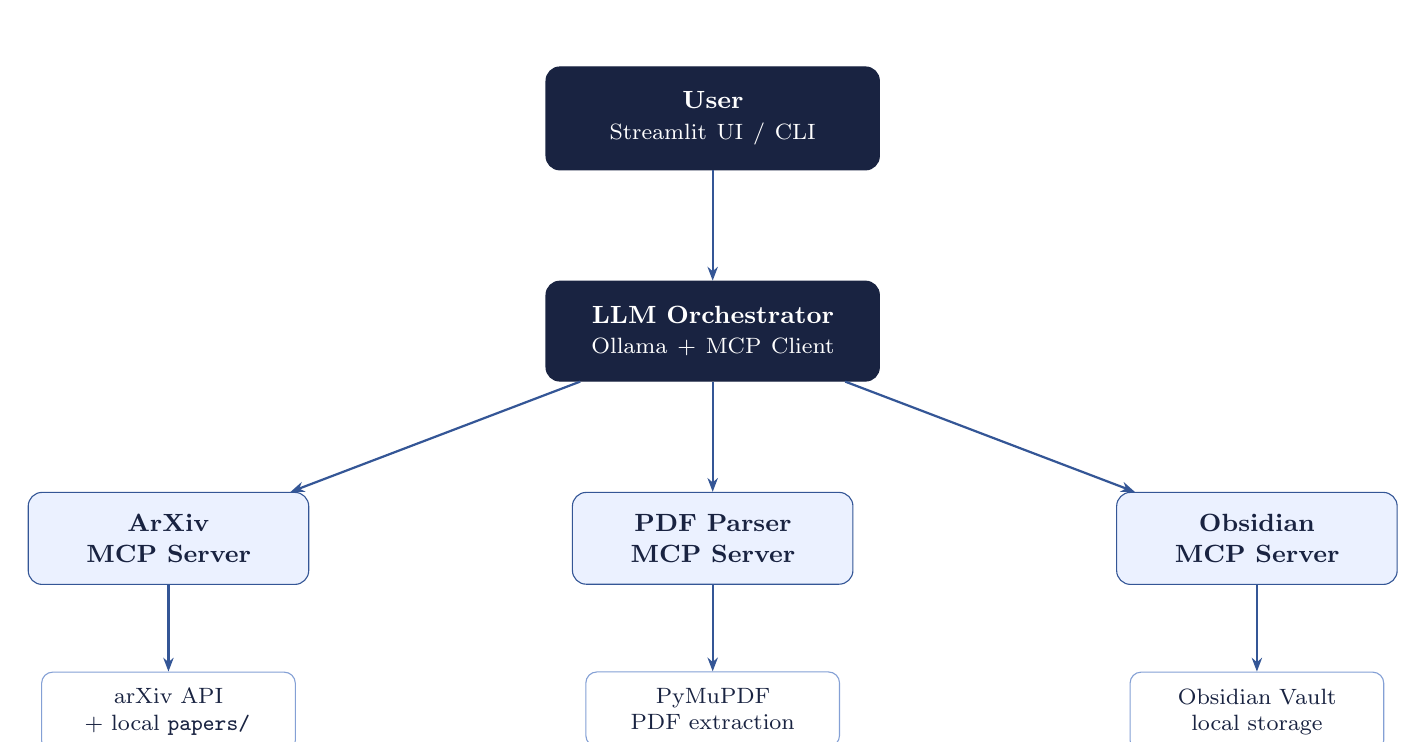
\begin{tikzpicture}[
    node distance = 1.5cm and 2.6cm,
    every node/.style = {font=\small},
    mainbox/.style = {
        rectangle, rounded corners=5pt,
        draw=darwindark, fill=darwindark,
        text width=3.6cm, align=center,
        inner sep=9pt,
        font=\small\bfseries\color{white}
    },
    serverbox/.style = {
        rectangle, rounded corners=5pt,
        draw=darwinblue, fill=darwinlight,
        text width=3.0cm, align=center,
        inner sep=8pt, font=\small\bfseries\color{darwindark}
    },
    storebox/.style = {
        rectangle, rounded corners=4pt,
        draw=darwinaccent!70, fill=white,
        text width=2.8cm, align=center,
        inner sep=6pt, font=\footnotesize\color{darwindark}
    },
    arr/.style = {-{Stealth[length=5pt]}, darwinblue, thick},
    label/.style = {font=\footnotesize\color{greytext}},
]

% Top: user
\node[mainbox] (user) {User\\{\footnotesize\normalfont\color{white}Streamlit UI / CLI}};

% Middle: orchestrator
\node[mainbox, below=1.4cm of user] (orch)
    {LLM Orchestrator\\{\footnotesize\normalfont\color{white}Ollama + MCP Client}};

% MCP servers
\node[serverbox, below left=1.4cm and 3.0cm of orch]  (arxiv) {ArXiv\\MCP Server};
\node[serverbox, below=1.4cm of orch]                  (pdf)   {PDF Parser\\MCP Server};
\node[serverbox, below right=1.4cm and 3.0cm of orch]  (obs)   {Obsidian\\MCP Server};

% Storage
\node[storebox, below=1.1cm of arxiv] (store1) {arXiv API\\+ local \texttt{papers/}};
\node[storebox, below=1.1cm of pdf]   (store2) {PyMuPDF\\PDF extraction};
\node[storebox, below=1.1cm of obs]   (store3) {Obsidian Vault\\local storage};

% Arrows
\draw[arr] (user)  -- (orch);
\draw[arr] (orch)  -- (arxiv);
\draw[arr] (orch)  -- (pdf);
\draw[arr] (orch)  -- (obs);
\draw[arr] (arxiv) -- (store1);
\draw[arr] (pdf)   -- (store2);
\draw[arr] (obs)   -- (store3);

\end{tikzpicture}
\captionof{figure}{High-level architecture of the Darwin system.}
\end{center}

\subsection{Layer Breakdown}

\subsubsection{Agent Orchestrator Layer}

The orchestrator (\code{src/agent/}) is the central reasoning engine. It initialises the Ollama language model client (\code{OllamaClient}) and the MCP session manager (\code{MCPClient}), then enters a multi-turn conversation loop. On each turn it:

\begin{itemize}[leftmargin=2em, itemsep=3pt]
    \item Sends the current message history and available tool schemas to the local LLM.
    \item Parses the model response for tool calls.
    \item Executes approved tool calls against the appropriate MCP server.
    \item Appends tool results to message history and re-invokes the model.
    \item Repeats until the model produces a final response with no further tool requests.
\end{itemize}

\subsubsection{Model Client Layer}

\code{OllamaClient} wraps the Ollama Python SDK. It accepts a model name, host URL, and optional system prompt at construction time and exposes a single \code{chat()} method that forwards messages and tool schemas to the Ollama \code{/api/chat} endpoint with \code{stream=False}. Switching the underlying model requires only a one-line config change.

\subsubsection{MCP Server Layer}

\code{MCPClient} manages connections to all configured MCP servers simultaneously using an \code{AsyncExitStack}. At startup it reads \code{config/claude\_desktop\_config.json}, opens a stdio transport session for each server, normalises their tool schemas into OpenAI-compatible function-calling format, and presents the merged tool list to the orchestrator.

% ══════════════════════════════════════════════════════════════════════════════
\section{Implementation}

\subsection{ArXiv MCP Server}

The ArXiv server (\code{src/arxiv\_server/server.py}) is built with FastMCP and exposes six tools covering the full paper lifecycle:

\begin{center}
\begin{tabular}{>{\ttfamily\small}l p{9cm}}
    \toprule
    \normalfont\textbf{Tool} & \textbf{Description} \\
    \midrule
    search\_papers       & Queries the arXiv API with a keyword string and a configurable result cap. Returns structured metadata: ID, title, publication date, summary, and PDF URL. \\[4pt]
    download\_paper      & Downloads a paper by arXiv ID to the local \code{papers/} directory. Checks for an existing cached file before making any network request. \\[4pt]
    list\_papers         & Returns a directory listing of all locally cached PDFs. \\[4pt]
    read\_paper          & Opens a local PDF with PyMuPDF and returns full page text. Bounded by a configurable character cap to protect the model's context window. \\[4pt]
    confirm\_download    & Formats paper metadata into a human-readable confirmation request and returns it to the orchestrator, which presents it to the user before any download is initiated. \\[4pt]
    log\_research\_action & Persists a timestamped action record (operation type, paper ID, result payload) to a local SQLite database (\code{research\_log.db}). \\
    \bottomrule
\end{tabular}
\end{center}

\begin{lstlisting}[style=terminal, caption={ArXiv MCP server startup and tool discovery}]
[INFO] Starting ArXiv MCP Server...
Connected to arxiv
Discovering tools...
Found 8 tools.
  - search_papers
  - download_paper
  - list_papers
  - read_paper
  - confirm_download
  - log_research_action
  - extract_pdf_sections
  - extract_figures
Agent ready. Type 'exit' to quit.
\end{lstlisting}

\subsubsection{Local Caching}

Before every download the server iterates \code{papers/} and returns the existing path if a file with a matching arXiv ID prefix is found. This eliminates redundant network calls across sessions and makes repeated experiments fully deterministic.

\subsubsection{Logging}

Every agent action is recorded via \code{log\_research\_action}. The SQLite schema is:

\begin{lstlisting}[style=pycode]
CREATE TABLE IF NOT EXISTS actions (
    timestamp TEXT,
    action    TEXT,
    paper_id  TEXT,
    result    TEXT
)
\end{lstlisting}

This creates an auditable trail that can be exported for debugging or post-run quality evaluation.

% ─────────────────────────────────────────────────────────────────────────────
\subsection{PDF Parser MCP Server}

The PDF parser (\code{src/pdf\_parser/server.py}) is a separate FastMCP server providing two tools:

\begin{itemize}[leftmargin=2em, itemsep=4pt]
    \item \code{extract\_pdf\_sections} --- opens a PDF with PyMuPDF and returns the full concatenated page text for downstream section-level analysis by the LLM.
    \item \code{extract\_figures} --- provides the interface for figure extraction (extensible for richer image output in future iterations).
\end{itemize}

Keeping this as a distinct server preserves a clean service boundary between the paper retrieval flow (arXiv server) and the document intelligence flow (PDF parser), allowing either to be swapped independently.

% ─────────────────────────────────────────────────────────────────────────────
\subsection{Agent Orchestrator}

\subsubsection{Multi-Turn Tool Execution Loop}

The core of Darwin's intelligence is the tool execution loop in \code{src/agent/main.py}. The loop is structured as a nested \code{while True} that continues invoking the model until it produces a response with no tool calls:

\begin{lstlisting}[style=pycode]
while True:                        # outer: user turns
    user_input = input("You: ")
    messages.append({"role": "user", "content": user_input})

    while True:                    # inner: agent reasoning
        response = ollama.chat(messages, tools=tools)
        tool_calls = response["message"].get("tool_calls", [])

        if not tool_calls:
            break                  # model finished reasoning

        for tc in tool_calls:
            result = await mcp_client.call_tool(
                tc["function"]["name"],
                tc["function"]["arguments"]
            )
            messages.append({"role": "tool", "content": str(result)})
\end{lstlisting}

This pattern supports compound tasks --- such as searching, selecting, downloading, and summarising several papers --- within a single user prompt, without requiring the user to manually chain commands.

\subsubsection{Argument Type Coercion}

The orchestrator includes a \code{convert\_tool\_arguments()} function that inspects each tool's JSON schema and casts string arguments to the correct Python type (integer, float) before passing them to MCP servers. This prevents type errors when the LLM serialises numeric arguments as strings.

\subsubsection{OllamaClient}

\code{OllamaClient} passes the complete message history and the full tool schema list to the Ollama API on every turn. Tool schemas are already in OpenAI function-calling format (normalised by \code{MCPClient}), so Ollama can natively select and invoke tools without any prompt engineering.

\subsubsection{MCPClient}

\code{MCPClient} opens a separate \code{stdio} transport session per configured server and manages them all through a single \code{AsyncExitStack}. Tool lookup resolves the correct server at call time by iterating active sessions, ensuring the orchestrator remains server-agnostic.

% ─────────────────────────────────────────────────────────────────────────────
\subsection{Human-in-the-Loop Approval}

Downloads are gated by a two-stage enforcement mechanism:

\begin{enumerate}[leftmargin=2em, itemsep=4pt]
    \item \textbf{Workflow gate.} The agent's system prompt instructs the model to always call \code{confirm\_download} before \code{download\_paper} for any keyword-driven search flow. The \code{confirm\_download} tool returns formatted paper metadata (title, ID, date, abstract preview) that the orchestrator displays to the user before requesting a \texttt{yes/no/skip} decision.
    \item \textbf{Safety net.} Even if the model skips the workflow gate, the orchestrator's \code{download\_paper} handler checks an \code{approved\_papers} set and blocks any unapproved ID with an explicit \texttt{BLOCKED} message fed back to the model.
\end{enumerate}

Users can opt out of the gate per-query by including the phrases \texttt{without approval} or \texttt{auto-download} in their message, or by providing a direct arXiv ID (e.g.\ \texttt{download 2306.04338v1}).

% ─────────────────────────────────────────────────────────────────────────────
\subsection{System Prompt \& Agent Persona}

The agent's behaviour is governed by the system prompt in \code{config/agent\_config.json}:

\begin{lstlisting}[style=pycode, language={}]
"You are Darwin, an AI research assistant.
 You help users search, download, and organize academic papers.

 Rules:
 - ALWAYS call tools to execute actions, never just describe them.
 - Direct paper ID (e.g. 'download 2306.04338v1'):
   call download_paper() immediately, no confirmation needed.
 - Keywords 'without approval' or 'auto-download':
   skip confirmation, download directly.
 - 'search and download' with no keywords:
   call confirm_download() first, then download_paper() if approved.
 - After search_papers returns results, list ALL papers with
   their ID, title, and a short summary. Never list only one."
\end{lstlisting}

This prompt locks Darwin into an action-first research persona, prevents the common failure mode of the model describing tool calls without executing them, and enforces consistent search result presentation.

% ─────────────────────────────────────────────────────────────────────────────
\subsection{Streamlit User Interface}

The Streamlit application (\code{ui\_app.py}) provides a graphical front-end that communicates with the agent as a subprocess via \code{agent\_wrapper.py}. The wrapper reads commands from \code{stdin} and writes tagged protocol lines (\code{AGENT\_RESPONSE:}, \code{TOOL\_EXECUTE:}, \code{TOOL\_BLOCKED:}, \code{TOOL\_CONFIRM:}, \code{AGENT\_END}) to \code{stdout}. The UI parses these tags to render structured output, paper cards, and confirmation dialogs without blocking the Streamlit event loop.

% ══════════════════════════════════════════════════════════════════════════════
\section{End-to-End Workflow}

A complete Darwin session follows this sequence:

\begin{enumerate}[leftmargin=2em, itemsep=5pt]
    \item \textbf{Startup.} The orchestrator loads \code{agent\_config.json}, initialises \code{OllamaClient} and \code{MCPClient}, connects to all configured MCP servers, and discovers the merged tool list.
    \item \textbf{Search.} The user submits a research topic. Darwin calls \code{search\_papers} and presents all results with IDs, titles, and one-line summaries.
    \item \textbf{Approval.} For each candidate paper the agent calls \code{confirm\_download}, displays the abstract preview, and waits for user confirmation.
    \item \textbf{Download \& cache.} Approved papers are fetched via \code{download\_paper} and saved to \code{papers/}. Subsequent runs retrieve them from cache without any network call.
    \item \textbf{Content extraction.} Darwin calls \code{read\_paper} or \code{extract\_pdf\_sections} to extract text, then synthesises a per-paper summary.
    \item \textbf{Knowledge persistence.} The agent calls the Obsidian server to create a structured note for each paper, applying tags by topic, method, and publication year, and linking to the local PDF path.
    \item \textbf{Logging.} Every action is written to \code{research\_log.db} via \code{log\_research\_action} for traceability.
    \item \textbf{Digest.} The agent produces a final digest note in Obsidian consolidating all findings from the session.
\end{enumerate}

\begin{lstlisting}[style=terminal, caption={Live agent session searching for interpretability papers}]
You: Find 3 recent papers on mechanistic interpretability in ML,
     then summarise each one.

Executing tool: search_papers...
Args: {'max_results': 3, 'query': 'mechanistic interpretability ML'}
Calling search_papers on arxiv...
[INFO] Found paper: 2306.04338v1
[INFO] Found paper: 1606.05386v1
[INFO] Found paper: 1806.09710v1
[INFO] Returning 3 results

Agent: Found 3 papers:

1. Model-Agnostic Interpretability of Machine Learning (1606.05386v1)
   Proposes a model-agnostic approach to explain ML predictions,
   enabling flexible choice of models and explanations.

2. Changing Data Sources in the Age of Machine Learning (2306.04338v1)
   Highlights risks when changing data sources in ML for official
   statistics --- emphasises robustness and data sourcing integrity.

3. Why Interpretability in Machine Learning? (1806.09710v1)
   Argues for human interpretability, characterises performance using
   distributed detection theory, shows interpretable classifiers
   outperform black-box ones.

Executing tool: confirm_download...
PAPER DOWNLOAD CONFIRMATION
  Title:     Model-Agnostic Interpretability of ML
  Paper ID:  1606.05386v1
  Published: 2016-06-16
  Abstract:  We propose LIME, a novel explanation technique that
             explains the predictions of any classifier...

Approve? (yes/no/skip): yes
Executing tool: download_paper... -> papers/1606.05386v1.pdf
Executing tool: log_research_action... -> research_log.db
\end{lstlisting}

% ══════════════════════════════════════════════════════════════════════════════
\section{Feature Summary}

\begin{center}
\renewcommand{\arraystretch}{1.4}
\begin{tabular}{p{4.2cm} p{8.0cm} l}
    \toprule
    \textbf{Feature} & \textbf{Description} & \textbf{Status} \\
    \midrule
    LLM Orchestrator      & Multi-turn tool execution loop via Ollama          & \done \\
    ArXiv MCP Server      & Search, download, list, and read papers            & \done \\
    PDF Parser Server     & Full-text and section extraction via PyMuPDF       & \done \\
    Obsidian Integration  & Structured note creation and vault management      & \done \\
    Streamlit UI          & Graphical interface with subprocess agent          & \done \\
    Human-in-the-Loop     & Two-stage approval gate for paper downloads        & \done \\
    Local Paper Cache     & File-based deterministic cache in \code{papers/}  & \done \\
    Logging \& Audit      & SQLite action log with full traceability           & \done \\
    Type Coercion         & Argument casting from LLM string output            & \done \\
    Error Handling        & \texttt{try/except} guards on all IO-heavy paths   & \done \\
    System Prompt         & Action-first research persona in agent config      & \done \\
    Multi-provider        & Swappable model backend via config                 & \done \\
    \bottomrule
\end{tabular}
\end{center}

% ══════════════════════════════════════════════════════════════════════════════
\section{Privacy \& Design Properties}

\begin{infobox}
\textbf{Data residency.} All paper PDFs, extracted text, Obsidian notes, and the action log are stored on the user's local filesystem. The only external communication is the arXiv public API (paper search and PDF download), which does not require authentication and does not receive user identity information.
\end{infobox}

\begin{infobox}
\textbf{Model isolation.} The language model runs on the local Ollama server (\texttt{http://localhost:11434}). No query text, paper content, or conversation history leaves the machine during inference.
\end{infobox}

\begin{infobox}
\textbf{Separation of concerns.} The three-layer architecture (orchestrator / model client / MCP servers) means that any layer can be audited or replaced independently. Researchers who want to switch from Ollama to a self-hosted API endpoint, or add a new data source, do so without modifying the other layers.
\end{infobox}

% ══════════════════════════════════════════════════════════════════════════════
\section{Conclusion}

Darwin delivers a complete, privacy-preserving research pipeline that operates from a single conversational interface. The combination of a local LLM, a modular MCP server layer, and a multi-turn agentic control loop enables autonomous literature review workflows that would otherwise require manual coordination across multiple tools.

The system is fully operational across all planned phases: the arXiv and PDF servers cover the retrieval and extraction pipeline; the Obsidian integration handles persistent knowledge management; the human-in-the-loop gate and local caching make the agent safe and efficient for repeated use; and the SQLite audit log provides the traceability needed for reproducible research workflows.

Darwin demonstrates that privacy-preserving agentic research assistants are achievable today, without cloud infrastructure, using open-source models and standard protocol primitives. The MCP-based design ensures the system will remain extensible as new data sources and tools become available.

\vspace{1.5em}
\begin{mdframed}[
    backgroundcolor = darwinlight,
    linecolor       = darwinblue,
    linewidth       = 1.5pt,
    innerleftmargin = 14pt,
    innerrightmargin= 14pt,
    innertopmargin  = 10pt,
    innerbottommargin= 10pt,
]
\textbf{Key insight.} The multi-turn tool execution loop in \code{src/agent/main.py} is the mechanism that transforms Darwin from a static question-answering chatbot into an agentic research workflow engine. Every other feature --- caching, approval gates, logging, Obsidian notes --- plugs into this loop as independently testable MCP tool calls.
\end{mdframed}

\end{document}
